%!TEX root = ../../thesis_master.tex

%%%%%%%%%%
\chapter{System Validation}
\label{chap:system-validation}
%%%%%%%%%%

In the present chapter the IBVS controller developed in this work will be validated. First, the performance of the system implementation will be tested.  Secondly, it will be validated if the system proposed satisfies the requirements described in Chapter \ref{chap:srs-sa}.

%%%%%%%%%%%%%%%%%%%%%%%%%
\section{Controller Performance}
\label{sec:controller-performance}
%%%%%%%%%%%%%%%%%%%%%%%%%

In this section, the performance of the proposed control scheme is verified experimentally by means of Gazebo simulations of an aerial robot. All the experiments were undertaken using the \texttt{hector\_quadrotor} aerial robot and the simulations run in the hardware configuration mentioned in Section \ref{sec:general-constraints}.

%%%%%%%%%%%%%%%%%%%%%%%
\subsection{Experimental Conditions}
\label{sec:experimental-conditions}
%%%%%%%%%%%%%%%%%%%%%%%

\begin{enumerate}
	\item \textbf{Prototype description}. The aerial robot used for the text is a quadrotor. The vehicle is equiped with an IMU that allow its state estimation and feed the low level controllers. Two low-level controllers take care of teh attitude stabillization and the velocity control. The camera used for the visual servoing task is placed on board of the quadrotor and pointg downwards towards the target. The 2D visual information comming from the camera is used as the only input for the visual servo controller running ontop of the low-level controllers. The visual controller sends velocity commands to the velocity controller to control kinematicaly the translational and the yaw degrees of freedom. The velocity commands of the quadrotor are saturated to ensure that it stays in quasi-stationary flight regime. In case that the linear velocity vector is bigger that 0.2 m/s, the vector is scaled to this limit value. For the yaw angular velocity a saturation of 0.2 rad/s, so the vehicle can rotate half-revolution in the usual convergence time.
	
	\item \textbf{Experimental environment}. For the simulation scenario the Gazebo's \texttt{empty\_world} is used. The illummination conditions are the standard conditions of this scenario, the only modification done to it is the target's placement and the robot's respawn. The target is placen in the origin of the \texttt{world} frame. The vehicle is navigated until its initial position using a joystick. The \texttt{tf}\footnote{\url{http://wiki.ros.org/tf}} transformations between the target's frame $T$ and the camera frame $C$ are used to ensure that the intitial pose is always correct.
	
	\item \textbf{Experimental protocol}. Once the robot is in the desired initial condition the action client for the controller is called. The user clicks on the target and the visual servoing starts. The controller publishes the current error through the action interface feedback. Additional data used for the performance evaluation is published using a custom menssage. The robot state used for the validation come from the real robot (simulatio) state that Gazebo publishes into the topic \texttt{/gazebo/model\_states}. All the interesting topics are recorded using\texttt{ rosbag}\footnote{\url{http://wiki.ros.org/rosbag}}. Then, a Python script is used to open the bag file and format the necessary data into comma separated values. The resulting files are porcessed with Python to produce the plots.
	
	The tunning of the PID's gains was conducted in the following form: the proportional gain is increased until convergence is achieved without too much overshoot. Then the integral and proportional gains are adjusted to reduce the oscillations. Empirically, these last gains must be around a hounded times smaller. Since they will work only when the error is very small and only small corrections are necessary.
	
	The sampling ration of the high-level visual servoing controller is limited to 20 Hz due to the bottleneck of the computer simulation without GPU. While Gazebo solves the physics ODEs using CPU computing, the camera simulations are run in this other component. In the optimal conditions the computer should be able to run the simulation until achieving a 50 Hz rate. In case of changing this rate, a new PID tuning would be needed.
	
	\nomenclature[ba]{GPU}{Graphics Processing Unit}
	\nomenclature[ba]{ODE}{Ordinary Differential Equation}
	\nomenclature[ba]{CPU}{Central Processing Unit}
	
	\item \textbf{Test cases}. Different initial conditions were considered to test the performance in all the possible cases and are presented below. For all the cases, the error convergence criteria used are $10^{-5}$ for the translation error and $5\times 10^{-3}$ for the rotational one.The first was chosen empirically to have millimeter accuracy in the final pose and the second ensures an orientation error of $10^{-4}$ rad $\simeq 0.3$ deg.
	
	Noisy camera input conditions were also test. It was founded that since all the feature computation is based on the AprilTag detection, it robustness makes that common camera Gaussian noise conditions ($\mu = 0$ and $\sigma = 0.1$) do not influence the results.
\end{enumerate}

%%%%%%%%%%%%%%%%%%%%%%%
\subsection{Large Initial Displacements}
\label{sec:large-initial-displacements}
%%%%%%%%%%%%%%%%%%%%%%%

For the case of large initial displacements the initial pose was chosen to be $(x, y, z) \simeq (-0.9, -0.5, 2.0)$ m and $(\phi, \theta, \psi) \simeq (0.0, 0.0, 18)$ deg. With desired pose $(x, y, z) \simeq (0.0, 0.0, 1.0)$ m and $(\phi, \theta, \psi) \simeq (0.0, 0.0, 0.0)$ deg (camera hovering over the target at 1 m height of the ground ). The results of this test case are presented in Figure \ref{fig:large-displacements} and identified with different letters form \emph{a} to \emph{f}.

%Different data has been plotted in the figure:
%
%\begin{itemize}
%	\item \emph{Visual error} $\bm{e}$:
%\end{itemize}

Due to the linear correspondence between image and task space, the system response shows a good asymptotic convergence for both image and task space. The convergence time being $t > 12$ s.

During the first second is possible to observe in the disturbance caused by the dynamic effects when the aerial robot is accelerating from zero to the commanded velocity. These dynamic effects are bigger in (\emph{e}) the actual robot's velocity achieved by the low-level controllers than in (\emph{c}) the commanded velocities by the high-level visual servoing.

Some oscillation still occurs before convergence, but this could be caused by the low-level controllers not being able to achieve in time the small velocities required (e.g. due to minimum velocity change of the motors and dynamic effects) for the final correction, since the accuracy imposed is very high.

The yaw control appears to oscillate a bit in (\emph{c}) the commanded velocities, although (\emph{e}) the achieved yaw angular velocity is very stable. The same happens in (\emph{f}), where the orientation with respect to the target converges exponentially asymptotically to the desired one. The small disturbances in $\phi$ and $\theta$ are due to the changes of speed at the beginning and during convergence. Since they stay small, the assumption of image plane parallel to the target plane is still valid.

\begin{figure}[!htb]
	\caption{Visual servo controller test results for large displacements}
	\centering
	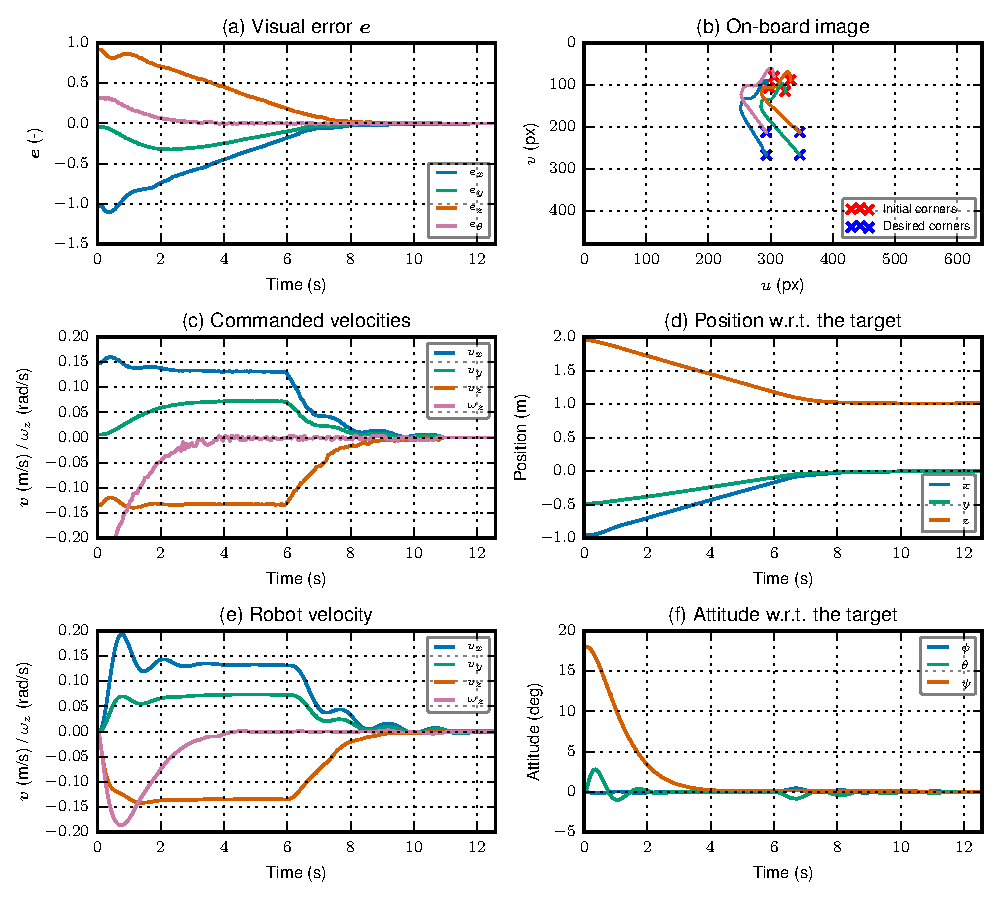
\includegraphics[width=\textwidth]{content/chapter_06/images/exp_015_plot.pdf}
	\label{fig:large-displacements}
\end{figure}

%%%%%%%%%%%%%%%%%%%%%%%
\subsection{Small Initial Displacements}
\label{sec:small-initial-displacements}
%%%%%%%%%%%%%%%%%%%%%%%

For the case of small initial displacements the initial pose was chosen to be $(x, y, z) \simeq (-0.2, 0.2, 1.4)$ m and $(\phi, \theta, \psi) \simeq (0.0, 0.0, 10)$ deg. With desired pose $(x, y, z) \simeq (0.0, 0.0, 1.0)$ m and $(\phi, \theta, \psi) \simeq (0.0, 0.0, 0.0)$ deg (camera hovering over the target at 1 m height of the ground ). The results of this test case are presented in Figure \ref{fig:small-displacements} and identified with different letters form \emph{a} to \emph{f}. The results here are similar to the large displacements case. Convergence time is lower here.

\begin{figure}[!htb]
	\caption{Visual servo controller test results for small displacements}
	\centering
	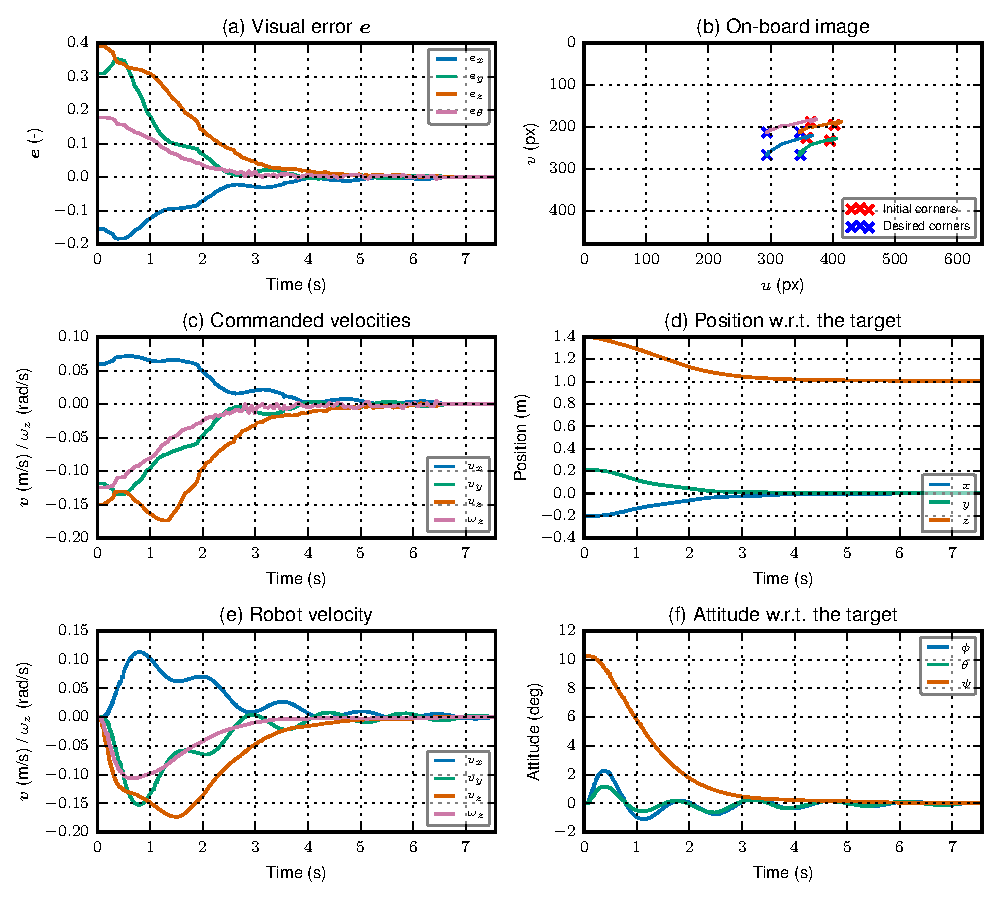
\includegraphics[width=\textwidth]{content/chapter_06/images/exp_017_plot.pdf}
	\label{fig:small-displacements}
\end{figure}

%%%%%%%%%%%%%%%%%%%%%%%%%
\section{Validation of the Requirements}
\label{sec:requirements-validation}
%%%%%%%%%%%%%%%%%%%%%%%%%

In this section, the requirements for the developed system, which where imposed in Section \ref{sec:srs} are validated.

%%%%%%%%%%%%%%%%%%%%%%%%%
\subsection{Validation of the Functional Requirements}
\label{sec:functional-requirements-validation}
%%%%%%%%%%%%%%%%%%%%%%%%%

In Section \ref{sec:functional-requirements}, five different functional requirements where imposed. Now, it is discussed whether each of them was satisfied:

\begin{itemize}
	\item \textbf{F1}: \emph{Compute desired visual features}. Chapter \ref{chap:system-design} describes how the ROS node \texttt{vs\_action\_server} computes the visual features from the desired pose and the known target dimensions.
	
	\item \textbf{F2}: \emph{Compute current visual features}. Chapter \ref{chap:system-design} describes how the ROS node \texttt{vs\_action\_server} computes the visual features from the current camera image and the detected target's corners.
	
	\item \textbf{F3}: \emph{Compute feature difference}. Once the current and desired features are computed, the same node computes its difference.
	
	\item \textbf{F4}: \emph{Provide velocity commands to the low level controller}. Once the desired camera velocities have been computed by the PID controller described in Chapter \ref{chap:implementation} are known, they are transformed to the robot's body frame $E$.
	
	\item \textbf{F5}: \emph{Provide feedback to the user and terminate the visual servoing task}. Thanks to the action interface described in Section \ref{sec:ros_action}, the user receives feedback about the current error in the controller, as well as notification when the task succeeded or it was preempted.
\end{itemize}

%%%%%%%%%%%%%%%%%%%%%%%%%
\subsection{Validation of the Qualitative Requirements}
\label{sec:sec:other-requirements-validation}
%%%%%%%%%%%%%%%%%%%%%%%%%

Section \ref{sec:other-requirements} described the qualitative requirements of the system proposed. Now, it is discussed whether each of them was satisfied:

\begin{itemize}
	\item \textbf{A1}: \emph{All components are working reliably}. The software has been tested using Gazebo simulations and its performance analyzed in Section \ref{sec:controller-performance}.
	
	\item \textbf{A2}: \emph{The software is sufficiently fast, modular and modifiable}. Modularity and modifiability has been greatly achieved thanks to the integration of the system in different ROS nodes and the use of an action interface to send tasks to the visual servoing high-level controller. Additionally, other visual features could be implemented thank to the use of the ViSP library.
	
	\item \textbf{A3}: \emph{The implementation is transparent and comprehensible}. The implementation has been comprehensively documented. 
	
	\item \textbf{A4}: \emph{Control inputs must provide stable and smooth flight maneuvers}. The controller's velocity commands are saturated so the velocities are slow enough to satisfy the assumption of the image plane been parallel to the target. Under this conditions the trajectory is exponentially asymptotic.
	
	\item \textbf{A5}: \emph{Robot must be able to start from different initial positions}. Different initial positions have been tested during the performance validation in Section \ref{sec:controller-performance}.
	
	\item \textbf{A6}: \emph{Algorithm must be fast enough to allow real time control of the aerial robot}. The software speed is not a problem. However, it has been identified a bottleneck for the test computer in the image simulation performed by Gazebo. The computer does not have a graphic performance enough to produce images at a rate higher that 20 Hz, thus limiting the controller to this rate, which still is enough to obtain the desired results.
	
	\item \textbf{A7}: \emph{The implementation should follow the style guide of ROS}. All the code has been conveniently formated and documented following the mentioned style guide.
\end{itemize}